
% Preamble
% ---
\documentclass[11pt,fleqn]{article}

% Packages
% ---
\usepackage[
  left=3cm,
  right=3cm,
  top=2cm,
  bottom=2cm]{geometry}
\usepackage{amsmath}
\usepackage{amssymb}
\usepackage{amsthm}
\usepackage{mathtools}
\usepackage{enumerate}
\usepackage{clrscode3e}
\usepackage{blkarray}
\usepackage{booktabs}
\usepackage{parskip}
\usepackage{mathptmx}
\usepackage{bigstrut}
\usepackage{caption}
\usepackage{mathptmx}
\usepackage{minted}
\usepackage[pdftex,pdfpagelabels,bookmarks,hyperindex,hyperfigures]{hyperref}
\usepackage{apacite}
\usepackage{tikz}
\usepackage{float}
\usepackage{graphicx}


% Use borland colorscheme in minted.
\usemintedstyle{borland}

% Replace outlined proof square with a black square.
\renewcommand\qedsymbol{$\blacksquare$}

% Document
% ---
\begin{document}

% Title
% ---
\title{Exploring the Traveling Salesman Problem}
\author{Brennan Hoeting}
\date{}
\maketitle

% Introduction
% ---
\section*{Introduction}
The Traveling Salesman Problem (TSP) is a classic NP---hard problem
in the field of computer science.  Like every other NP--hard problem,
it can only be solved in exponential runtime, or approximated in polynomial
runtime.  In this paper, we will obtain an understanding of the TSP problem
by explaining what it is, examining its input and output, and looking at
different algorithms that can obtain or approximate a solution.  We will
present and explain a naive brute force solution to the problem and analyze
its efficiency.  Then we will look at alternative TSP algorithms and discuss
the use cases and advantages of each approach.  We will choose one of the
algorithms and present its pseudocode, as well as detailed mathematical
notation to gain a better understanding of how it computes the solution.

\section{Understanding the Problem}
\subsection{Overview}
The traveling salesman problem can be described as follows:
Given a set of cities, where there is a distance between
each pair of cities, find a tour (route) that begins at a
\textit{starting city}, visits each \textit{destination city}
exactly once, and returns to the starting city covering the minimum
possible total distance.  We will refer to the tour with the
minimum possible distance traveled as the \textit{optimal tour}.

\subsection{Problem Input}
The problem input is a matrix that defines the distance
between each pair of cities.  We will refer to this as
a \textit{distance matrix} or \textit{cost matrix} and denote
it as $D = (d_{ij})$, where $d_{ij}$ is the distance between city
$i$ and city $j$.  If the cost (distance) from city $i$ to city $j$
is equal to the cost from city $j$ to city $i$ then the TSP variation
is \textit{undirected} and our distance matrix is symmetric.
\par

An example of a \textit{directed} variation of the TSP is one that
optimizes for minimum total airfare to travel a tour by plane,
where ticket prices from city $i$ to city $j$ is not necessarily
equal to the ticket price from city $j$ to city $i$, implying the
cost matrix is asymmetric.
\par

Most exact TSP algorithms can solve both directed and undirected variations,
while approximation TSP algorithms can typically only solve undirected
variations.
\par

See the figure below for a valid input distance matrix for an undirected
TSP variation.  Notice, for example, that the distance between city $1$
and city $4$ is $d_{1,4}=d_{4,1}=29$.  If we ran into a case while
implementing a TSP algorithm
\par

\begin{align*}
  d_{ij}=
  \begin{blockarray}{cccccc}
    & j_1 & j_2 & j_3 & j_4 & j_5 \\
  \begin{block}{c(ccccc)}
    i_1 & 0 & 7 & 37 & 29 & 17 \\
    i_2 & 7 & 0 & 31 & 32 & 34 \\
    i_3 & 37 & 31 & 0 & 32 & 42 \\
    i_4 & 29 & 32 & 32 & 0 & 20 \\
    i_5 & 17 & 34 & 32 & 20 & 0 \\
  \end{block}
  \end{blockarray}
\end{align*}

It is common to describe the input of the TSP as a complete graph.
We define the graph as $G=(V,E)$, where $v_i$ is the $i^{\text{th}}$
city and $e_ij$ is the distance between city $i$ and city $j$.  Below
is an example what such a graph could look like:

\tikzstyle{vertex}=[circle, draw, minimum size=1.2cm]
\tikzstyle{edge}=[draw=black]
\begin{tikzpicture}[shorten >=1pt, auto, node distance=7cm]
  \node[vertex](v1) at (6, 4) {$ v_1 $};
  \node[vertex](v2) at (11, 2) {$ v_2 $};
  \node[vertex](v3) at (10, -2) {$ v_3 $};
  \node[vertex](v4) at (2, -2) {$ v_4 $};
  \node[vertex](v5) at (1, 2) {$ v_5 $};

  \draw[edge] (v1) edge node{\scriptsize 7}  (v2);
  \draw[edge] (v1) edge node{\scriptsize 37} (v3);
  \draw[edge] (v1) edge node{\scriptsize 29} (v4);
  \draw[edge] (v1) edge node{\scriptsize 17} (v5);

  \draw[edge] (v2) edge node{\scriptsize 31} (v3);
  \draw[edge] (v2) edge node{\scriptsize 32} (v4);
  \draw[edge] (v2) edge node{\scriptsize 34} (v5);

  \draw[edge] (v3) edge node{\scriptsize 32} (v4);
  \draw[edge] (v3) edge node{\scriptsize 42} (v5);
  
  \draw[edge] (v4) edge node{\scriptsize 42} (v5);
\end{tikzpicture}

\subsection{Problem Output}
A common output for a TSP is a matrix with the dimensions $N\times N$, where
$N$ is the number of cities.  We can define the output as the edge matrix
$E = (e_{ij})$, where $e_{ij}=1$ if the optimal tour involves
traveling from city $i$ to city $j$.  $e_{ij}=0$ if meaning we will not
travel from city $i$ to city $j$ along the optimal tour.
\par

Below is an example of a valid edge matrix output for our TSP variation.
Notice that $e_{3,4}=1$ implying our optimal tour involves traveling from
city $3$ to city $4$.  Since this output is for an undirected TSP instance,
$e_{4,3}$ is also $1$.
\par

\begin{align*}
  e_{ij}=
  \begin{blockarray}{cccccc}
    & j_1 & j_2 & j_3 & j_4 & j_5 \\
  \begin{block}{c(ccccc)}
    i_1 & 0 & 1 & 0 & 0 & 1 \\
    i_2 & 1 & 0 & 1 & 0 & 0 \\
    i_3 & 0 & 1 & 0 & 1 & 0 \\
    i_4 & 0 & 0 & 1 & 0 & 1 \\
    i_5 & 1 & 0 & 0 & 1 & 0 \\
  \end{block}
  \end{blockarray}
\end{align*}

TSP algorithms can also output a graph $G=(V,E)$, where $V_i$
represents city $i$ and $E_{ij}$ represents traveling from city $i$ to
city $j$ along the optimal tour, where the weight is the distance between
the two.  If the graph where visualized, each vertex would be positioned
at its longitude and latitude coordinates and a segment would connect each pair
of vertices $v_i$ and $v_j$ where $e_{ij}=1$.  The single path in the graph
represents the optimal tour.
\par

\tikzstyle{vertex}=[circle, draw, minimum size=1.2cm]
\tikzstyle{edge}=[draw=black]
\begin{tikzpicture}[shorten >=1pt, auto, node distance=7cm]
  \node[vertex](v1) at (6, 4) {$ v_1 $};
  \node[vertex](v2) at (11, 2) {$ v_2 $};
  \node[vertex](v3) at (10, -2) {$ v_3 $};
  \node[vertex](v4) at (2, -2) {$ v_4 $};
  \node[vertex](v5) at (1, 2) {$ v_5 $};

  \draw[edge] (v1) edge node{\scriptsize 7}  (v2);
  \draw[edge] (v2) edge node{\scriptsize 31} (v3);
  \draw[edge] (v3) edge node{\scriptsize 32} (v4);
  \draw[edge] (v4) edge node{\scriptsize 42} (v5);
  \draw[edge] (v5) edge node{\scriptsize 17} (v1);
\end{tikzpicture}

Another way to represent the optimal tour is with a list
$T$, where for every $i \lte n$, $(i-1, i)$ represents
traveling from city $i-1$ to city $i$ along the optimal
tour.  This paper will primarily use this type of output.


\section{A Naive Brute Force Algorithm}
\subsection{Overview}
The brute force method for solving the Traveling Salesman Problem has exactly
two redeeming qualities: (1) it is quite simple, making implementation
trivial, and (2) it will produce the correct tour in every TSP instance.
Unfortunately, for instances that contain more than roughly 20 cities, the
algorithm does not finish execution in a reasonable time.  Analyzing the
pseudocode in (2.2), we can get a good idea of why this is the case.
\par
\vspace{0.5cm}


\subsection{Pseudocode}
\begin{codebox}
\Procname{$\proc{OPTIMAL-TOUR}(D:$ distance matrix$)$}
\li $\id{T} \gets$ all permutations of $[2 \twodots \attrib{D}{length}]$
\li $\id{min-dist} \gets \infty$
\li $\id{min-tour} \gets \const{nil}$
\li \For each tour $t \in T$
\li   \Do
        $\id{t} \gets [1] + T + [1]$
\li       $\id{dist} \gets \proc{TOUR-DISTANCE}(D, t)$
\li	  \If $dist < \id{min-dist}$
\li	    \Then
              $\id{min-dist} \gets dist$
\li	      $\id{min-tour} \gets tour$
            \End
       \End

\li    \Return $\id{min-tour}$
\end{codebox}
 
On line $1$, we assign $\id{T}$ to a list containing each permutation of
the seed list $[2 \twodots \attrib{D}{length}]$.  Each list $T_k$ represents
a partial tour such that $T_{k,i+1}$ is visited from $T_{k,i}$.  Each element
$T_{k,i}$ in $T_k$ corresponds to a row index $i$ in the distance matrix $D$.
\par

Notice that we initially exclude our starting city, $1$, from the seed list.
This is to ensure $T$ only includes permutations the destination cities. Next,
for each permutation $t$ in $T$, we append $1$ to the front and back of $t$.
This gives us a complete tour, starting on $1$, visiting each destination
exactly once, and ending on $1$.  Now we may calculate the total distance,
$\id{dist}$, of $t$ by calling the $\proc{TOUR-DISTANCE}(D, t)$ procedure,
which is simply:

\vspace{.27cm}
\hrule
\begin{codebox}
\Procname{$\proc{TOUR-DISTANCE}(t:$ tour, $D:$ distance matrix$)$}
\li $\id{dist} \gets 0$
\li \For $\id{i} \gets 2$ to $\attrib{t}{length}$
\li   \Do
$\id{dist} \gets \id{dist} + D_{i-1,i}$
       \End
\li    \Return $\id{dist}$
\end{codebox}
\vspace{.1cm}
\hrule
\vspace{.05cm}

If $\id{dist} < \id{min-dist}$, we update
$\id{min-dist}$ and $\id{min-tour}$.  Once the loop is finished, we
return the optimal tour.
\par


\subsection{Runtime}
Looking at the table below, we can see how the number of potential optimal
paths increases as the number of cities increases.
\par

\bgroup
\def\arraystretch{1.25}
\begin{tabular}{c|r}
  Cities $n$ & Possible Tours $(n-1){!}$ \\
  \hline
  \begin{tabular}{c}
    $4$ \\
    $5$ \\
    $\dots$ \\
    $10$ \\
    $11$ \\
    $12$
  \end {tabular}
  &
  \begin{tabular}{r@{\;{=}\;}l}
    $(4-1){!}$ & $6$ \\
    $(5-1){!}$ & $24$ \\
    $\dots$ & $\dots$ \\
    $(10-1){!}$ & $362,880$ \\
    $(11-1){!}$ & $3,628,800$ \\
    $(12-1){!}$ & $39,916,800$
  \end{tabular}

\end{tabular}
\egroup

The runtime of this method is upper bounded by the amount
of time it takes to generate each possible tour, so we can
say the algorithm is $O((n-1)!) = O(n!)$, where $n$ is the
number of cities.
\par


\section{A Better Algorithm}
\subsection{Overview}
While the brute force algorithm is simple and correct, it
is far too slow for larger inputs.  Fortunately, there are multiple
alternative TSP algorithms with a runtime
that is better than $O(n!)$.  We will explore in detail the
\textit{Held--Karp} algorithm, an $O(n^2 2^n)$ solution that uses
dynamic programming \cite{heldkarp}.  Then we will look at the Nearest
Neighbor algorithm and Christofides algorithm, both of which are polynomial
time approximation algorithms.  We will and discuss the advantages
and drawbacks of each approach. 

\subsection{Held--Karp}
The Held--Karp algorithm is an $O(n^2 2^n)$ approach to solving the TSP\@.
It is not fast enough to solve TSP instances with a large number of
cities, but the solution for the instances it can solve is guaranteed
to be correct.  The algorithm works as follows:
\par

Suppose $D = (d_{ij})$ is distance
matrix where $d_{ij} = d_{ji}$, $n$ is the number of rows in $D$,
$S$ is a subset of $\{1, 2,\dots,n\}$, and $x\in S$.  We define $C(S, x)$
to be the distance of the optimal tour that starts at $x$, visits each
destination exactly once, and ends at $1$ \cite{heldkarp}.  The recurrence
for $C(S,x)$ is:

\begin{align*}
  C(S, x)=\begin{cases}
    \min\{k\in S-\{x\} : d_{kx} + C(S-\{x\}, k) \}  & \text{if } n>1 \\
    d_{1x}                                          & \text{if } n=1
  \end{cases}
\end{align*}

We obtain the optimal cost from a distance matrix $D$ of size $n$ by calling
$C(\{1,\dots,n\}, 1)$.  We can apply dynamic programming principles to this
problem by storing the cost for each call in a lookup table $H$.  In each
recurrence where $n>1$, if the tuple $(S, x)$ exists in $H$, we can return
$H[(S, x)]$.  Otherwise,  we will compute the cost and store it in $H$.
\par

This alone does not solve the original problem.  We still need to return 
the optimal tour, not just its distance.  We can find the optimal tour
by using an additional lookup table, $P$, that maps $(S, x)$ to the optimal
$(S-\{x\}, k)$ at each step.  We can obtain the final optimal tour by
backtracking through $P$.  We define the optimal tour as $T$ and $B(v)$ as a
recurrence that backtracks through $P$:

\begin{align*}
  B(v)=\begin{cases}
    B(P[v])     & \text{if } v \text{\ in\ } P \\
    \const{nil} & \text{otherwise} 
  \end{cases}
\end{align*}

We fill in the values of $T$ by calling $B((\{1,\dots,n\}, 1))$.  On each
recurrence where $v$ is in $P$, we append the second value in $v$ (the $k$
value) to $T$.  When $v$ is not in $H$ and $\const{nil}$ is returned
from $B(v)$, we append $1$ to $P$, resulting in the optimal tour.
\par

\subsection{Christofides}
Christofide's algorithm is an $O(n^3)$ approximation algorithm that guarantees
the cost of its solution will be strictly within $3/2$ of the optimal solution
cost.  The algorithm only works on a symmetric distance matrix that satisfies
the triangle inequality \cite{nicos}.  That is, a distance matrix $D=d_{ij}$
may be used if the shortest path to reach every $j$ from
$i$ involves traveling directly to $j$ from $i$, rather than through a path that
includes more than two vertices.
\par

The algorithm works as follows: Given a distance matrix $D=d_{ij}$ and size $n$,
let $G=(V,E)$ where $v_i=i$ for all $i\in [1,\dots,n]$ and $e_{ij}=d_{ij}$.  The
optimal tour starting at $v_1$ is obtained using the following steps:
\begin{enumerate}
  \item Generate a minimum spanning tree, $MST$, rooted at $v_1$ using Prim's algorithm.
  \item Perform a preorder traversal on $MST$ and append the vertices in the order they 
    are visited to list a $T$.
  \item For each vertex in $T$, append it to $T'$ only when it is first visited.  This 
    removes duplicates from $T$ resulting in the optimal tour.
\end{enumerate}

The last step holds since $G$ satisfies the triangle inequality. \cite{nicos}

\subsection{Nearest Neighbor}
The Nearest Neighbor algorithm is a greedy approximation algorithm
for solving the TSP\@.  It starts at an arbitrary city, then visits
the closest city until each city has been visited once.  After each
visit, the city is added to the optimal tour $T$.  Once each node
has been visited, the starting city is appended to $T$ and $T$ is
returned. \cite{bellmore}
\par

The steps for this algorithm are as follows:
\begin{enumerate}
  \item Pick a starting city $s$, let it be the current city $x$.
  \item Add $x$ to the optimal tour $T$ and mark $x$ as visited.
  \item Determine the closest unvisited city $y$ from $x$.  If no
    unvisited cities exist, goto step 5.
  \item assign $x$ to $y$, repeat step 2.
  \item Add $s$ to $T$, return $T$.
\end{enumerate}

This is an $O(n^2)$ algorithm because on each iteration the
current city visits every other unvisited city.

\subsection{Comparing the Three}
We have examined one exact algorithm -- Held-Karp -- and two approximation
algorithms --Christofides and Nearest Neighbor.  The approximation algorithms
have the advantage of being significantly faster than the Held-Karp algorithm,
but they aren't applicable in every case, and they don't always return the optimal
tour for cases in which they are applicable.  The Held-Karp algorithm, on the other
hand, will return the optimal tour in every TSP instance, provided the number of
cities is small enough to allow the algorithm to finish execution in a reasonable
time.
\par

Christofide's algorithm and the Nearest Neighbor algorithm both perform at an
acceptable level (that is, they return the optimal tour enough of the time) for
Euclidean TSP instances \cite{gutin}.  If a TSP instance is Euclidean, then it satisfies the
triangle inequality.  This property is necessary for Christofide's algorithm to
return the correct tour \cite{nicos} and it greatly increases the probability
that the Nearest Neighbor algorithm will as well \cite{gutin}.
\par

For asymmetric and general symmetric TSP instances, Christofide's algorithm will
never return the optimal tour.  The Nearest Neighbor algorithm, on the other hand,
can find an optimal tour, but it's highly unlikely.  Additionally, for every $n \geq 2$
there exists at least one asymmetric or general symmetric TSP instance for which the
Nearest Neighbor algorithm returns the \textit{worst} tour. \cite{gutin}.  We are
optimizing for correctness over speed and problem size in this paper and will continue
to explore the Held--Karp algorithm.

\subsection{Held-Karp Pseudocode}
Below is the Pseudocode for the Held-Karp algorithm.  It is an iterative
dynamic programming implementation of the recurrence we defined in (3.2).
It uses two lookup tables, $C$ and $P$, for computing the optimal distances
and backtracking to obtain the optimal path, respectively.
\par

\vspace{.27cm}
\hrule
\begin{codebox}
\Procname{$\proc{HELD-KARP}(D:$ distance matrix$)$}
\li $\id{n} \gets \attrib{D}{length}$
\li $\id{C} \gets$ a lookup table that maps $(S, x)$ to the optimal cost
\li $\id{P} \gets$ a lookup table that maps $(S, x)$ to the optimal $(S-\{x\}, k)$
\li
\li \For $\id{k} \gets 2$ to $n$
\li   \Do
	$\id{C} \gets D_{1k}$
\li     $\id{P} \gets (\{\}, 1)$
      \End
\li
\li \For $\id{size} \gets 2$ to $n$
\li   \Do
	\For $\id{x} \gets 1$ to $n$
\li	  \Do
	    \If $size \isequal n$ and $x \neq 1$
\li	      \Then
		\textbf{continue}
	      \End
\li	    \For $\id{S} \gets \proc{SUBSETS}(\{2,\dots,n\}, size)$
\li	      \Do
		$\id{opt-k} \gets \const{nil}$
\li		$\id{opt-dist} \gets \infty$
\li		$\id{opt-subset} \gets \const{nil}$
\li		\For $k$ in $S-\{x\}$
\li		  \Do
		    $\id{dist} \gets \id{C}[(S-\{x\}, \id{k})] + D_{xk}$
\li		    \If $dist < \id{opt-dist}$
\li		      \Then
			$\id{opt-k} \gets k$
\li			$\id{opt-dist} \gets dist$
\li			$\id{opt-subset} \gets S$
		      \End
		  \End
\li
\li		  $\id{C}[(subset, x)] \gets opt-dist$
\li		  $\id{P}[(subset, x)] \gets (opt-subset, opt-k)$
	      \End
	  \End
      \End

\li
\li $T = []$
\li $\id{v} \gets (\{1,\dots,n\}, 1)$
\li \While $\id{v} \neq \const{nil}$
\li   \Do
	$\proc{\attrib{T}{append}}(v[2])$
\li	$\id{S} \gets \id{T}[v]$
      \End	
\li
\li \Return \id{T}
\end{codebox}
\vspace{.27cm}
\hrule

On lines 5-7, we add our base cases to the lookup tables.  In the main loop on
lines 9-25, we build the lookup tables in a bottom-up dynamic programming fashion.
Notice on lines 11 and 12 we continue when the subset size is $n$ and $x \neq 1$.
This achieves the effect of beginning our recurrence from (3.2) with $(\{1,\dots,n\}, 1)$,
ensuring we're only computing optimal paths that start at $1$.  Finally, on lines 27-31
we backtrack through our lookup table $P$ that stores the optimal $(S-\{x\}, k)$
for a given $(S, x)$, appending each optimal $k$ value to the optimal tour $T$.

\subsection{Held-Karp Runtime}
We will show that the Held-Karp algorithm is an improvement over the brute force
approach by proving the runtime of Held-Karp is $O(n^{2}2^n)$, which is better than
the runtime of brute force, $O(n!)$.

Observe from the pseudocode that our algorithm iterates from $2$ to $n$.  In that
loop we also iterate from $1$ to $n$.  This is where the $n^2$ portion of our runtime
comes from.  Also observe that the algorithm involves computing every possible subset
of $\{1,\dots,n\}$, where $n$ is the number of cities.  Knowing this, we can prove the
runtime by proving a set with $n$ elements has $2^n$ subsets using induction.

\begin{proof}
  (Induction) For our basis step, consider that an empty set $\varnothing$ has $1$
  subset (itself).  $2^n = 2^0 = 1$, so a set with $0$ elements has $2^0$ subsets.\
  For induction, suppose a $k$-element set has $2^k$ subsets.  We will show every
  $(k+1)$-element subset has $2^(k+1)$ subsets.  Let $A=\{a_1,a_2,\dots,a_k, b\}$,
  notice it contains $k+1$ elements.  We partition the subsets of $A$ into two sets
  $B$ and $C$, where $B$ contains the subsets that contain $b$ and $C$ contains
  the subsets that don't contain $b$.  $C$ contains every subset of $A-{b}$, so it
  has $2^k$ elements.  By construction, it follows that $B$ must have the same number
  of elements as $C$, so it also has $2^k$ elements.  Since $B$ and $C$ are independent
  sets, the size of $B\union C$ is $2^k + 2^k = 2^{k+1}$.
\end{proof}

\section{Experimental Comparison}

\subsection{Overview}
We will do an experiment on the brute force and Held--Karp algorithms,
running Python implementations of both algorithms and comparing their
execution times.

\subsection{Input}
The input for both algorithms will be a standard TSPLIB sample instance, as shown
in the table below.  The distance matrix is created using the $x$ and $y$ coordinates
in the table and is used by both algorithms to generate the optimal tour.
\par

\begin{table}[H]
  \centering
  \caption*{TSPLIB xqf131 input}
  \begin{tabular}{c|c|c}
    \toprule
    City & $x$ & $y$ \\
    \midrule
    1& 0& 13 \\
    2& 0& 26 \\
    3& 0& 27 \\
    4& 0& 39 \\
    5& 2& 0\\
    6& 5& 13\\
    7& 5& 19\\
    8& 5& 25\\
    9& 5& 31\\
    10& 5& 37\\
    11& 5& 43\\ 
    12& 5& 8\\ 
    13& 8& 0\\
    14& 9& 10\\
    15& 10& 10\\
    16& 11& 10\\
    17& 12& 10\\
    18& 12& 5\\
    \bottomrule
  \end{tabular}
\end{table}

\subsection{Execution}
We run both algorithms on the data set above and produce the runtime table
below.  Note that the brute force times for $n>10$ are estimated as the
algorithm takes too long to run for those problem sizes.
\par

\begin{table}[H]
  \centering
  \caption*{Runtime comparison}
  \begin{tabular}{c|c|c|c}
    \toprule
    Cities $n$ & Brute Force (s) & Held-Karp (s) & BF/HC \\
    \midrule
    4   &       0.00003       &    0.00005    &      0.60748      \\
    5   &       0.00010       &    0.00011    &      0.89353      \\
    6   &       0.00062       &    0.00032    &      1.94113      \\
    7   &       0.00437       &    0.00091    &      4.77795      \\
    8   &       0.03484       &    0.00226    &      15.37989     \\
    9   &       0.29779       &    0.00568    &      52.38270     \\ 
    10  &       2.84006       &    0.01420    &     199.93426     \\
    11  &       31.24068      &    0.03465    &     901.55505     \\
    12  &      374.88817      &    0.09049    &    4,143.09304    \\
    13  &     4,873.54623     &    0.24270    &    20,080.92283   \\
    14  &     68,229.64716    &    0.60574    &   112,639.24419   \\
    15  &   1,023,444.70737   &    1.44135    &   710,060.87550   \\
    16  &   16,375,115.31784  &    3.43850    &  4,762,288.58166  \\
    17  &  278,376,960.40329  &    8.09218    &  34,400,754.72416 \\
    18  & 5,010,785,287.25922 &    19.04262   & 263,135,354.10685 \\
    \bottomrule
  \end{tabular}
\end{table}

\subsection{Output}
The output from running the Held-Karp algorithm for 18 cities is a
list representing the optimal path:
$(1, 2, 3, 4, 11, 10, 9, 8, 7, 6, 14, 15, 16, 17, 18, 13, 5, 12, 1)$

Our program can also produce a graph:

\centering
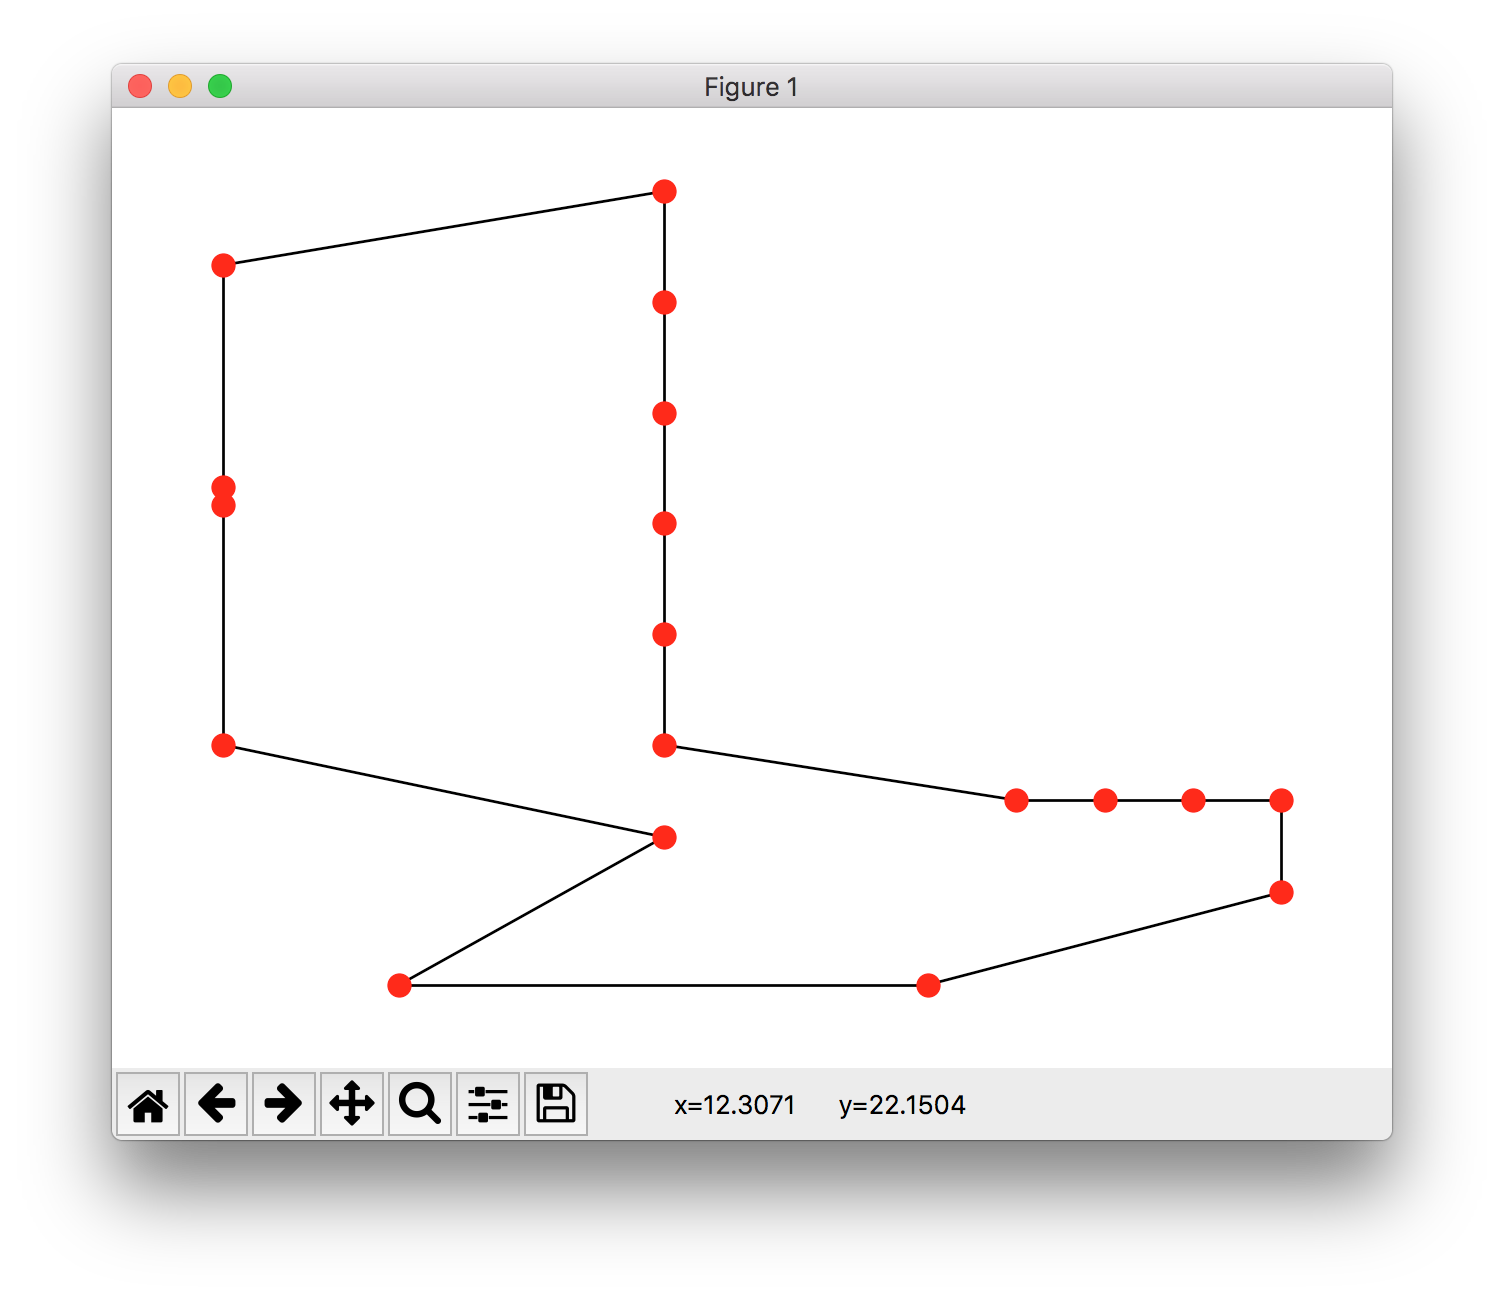
\includegraphics[scale=0.5]{plot.png}


\newpage
\appendix
\section*{Appendices}
\newpage
\addcontentsline{toc}{section}{Appendices}
\renewcommand{\thesubsection}{\Alph{subsection}}

\subsection{Collaboration}
  I collaborated with on this project Grant Eaton and Luke Artnak.
  \par

  Grant helped me search for primary sources to use in this paper.
  He also made a suggestion
  for space optimization on my Held-Karp implementation, which
  I agreed with, but did not implement.  I helped Grant
  with various Latex tasks and getting Python networkx code
  to work.

  Luke helped me analyze the runtime of the Held-Karp algorithm,
  which helped me greatly in writing the runtime proof.  He also
  made some suggestions on how I could make my Held-Karp python code
  more readable, which again, I did not follow through with.  I helped
  Luke get python networkx code working, although he ended up
  switching to JavaScript later on.

  \par

\newpage
\subsection{Source Code}
  Brute Force Implementation
  \inputminted[linenos=true]{python}{../src/brute_force.py}
  \newpage
  Held-Karp Implementation
  \inputminted[linenos=true]{python}{../src/held_karp.py}
  The output of the main program running on my machine.
  Yellow values are estimations.
  \includegraphics[scale=0.5]{screenshot.png}

\newpage
\subsection{Requirements}
For each of the requirements of the paper, I have given
the section where that requirement was met.
\begin{enumerate}
  \item Requirement: Describe the problem.  See sections 1.1, 1.2, and 1.3.
  \item Requirement: Explain your naive / BF implementation.  See section 2.
  \item Requirement: Motivate a solution that improves on the naive solution.
    See section 3.2 for better solution and 3.5 for a comparison.
  \item Requirement: Defend your solution against prior art: All of section
    3 contains cited work, primarily in section 3.5.
  \item Requirement: explain your improved solution by presenting pseudocode.  See section 3.6.
  \item Requirement: Provide a proof that your solution has some nontrivial property.  See section 3.7.
  \item Requirement: Experimentally compare your solution to BF / Naive approaches.  See section 4.
  \item Requirement: Do version A or B of the assignment.  I've done A by choosing the Held-Karp algorithm.
    Section 3.5 is explicitly states this paper is concerned with correctness, rather than speed.
\end{enumerate}

\newpage
\bibliographystyle{apacite}
\bibliography{biblio}

\end{document}
